\chapter{Diurnal Shift}
\label{chap:diurnalshift}
\begin{strip}
	\begin{minipage}{\textwidth}
		\begin{abstract}
			I present an improved model of diurnal shift, aiming to resolve issues evident in previous models and be more mathematically rigorous. I investigate the apparent sine-function variability of hourly meteor counts, as well as the temporal and spatial variation of said counts. My findings indicate that diurnal shift is dependent on Earth's orbital velocity, producing a clear trend between longitude and peak hour. I find no evidence of correlation between latitude and amplitude of diurnal variation.
		\end{abstract}
	\end{minipage}
\end{strip}
\section{Background}
For years, a notable increase and decrease over a single days' time scale has been observed in detection counts. An example of this is in figure~\ref{fig:data:rmob:b}. The red colours indicate a higher detection count, observed in the early hours of the morning. This diurnal shift {\it has} been given an explanation by modelling the phenomenon. The word `diurnal' refers to the time scale being a single day, and `shift' refers to the increase in detection counts. 
\section{Literature Review}
\subsection{Model}
Dr David Morgan of the BAA Radio Astronomy Group presents a somewhat detailed explanation \cite{baa} of why diurnal shift occurs. The suggestion is that diurnal shift is dependent on sporadic meteors rather than shower meteors, and depends on the variation of their intercept velocity with an observer on Earth. This changes since, as the Earth rotates, the combination of the orbital velocity, rotational velocity and meteor intercept velocity changes. As can be seen in figure~\ref{fig:dishift:model} (courtesy of the same article \cite{baa}), at Sunrise, the meteors velocity {\it adds} to Earth's orbital velocity, whilst at Sunset, these velocities {\it subtract}. 
\begin{figure}[h!]
	\centering
	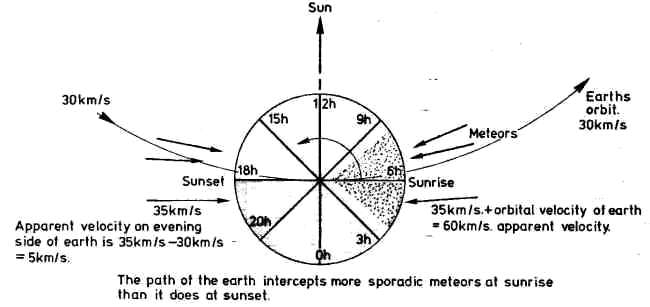
\includegraphics[width=\linewidth]{dishift/img59}
	\caption{Diurnal shift model
		\label{fig:dishift:model}}
\end{figure}
\subsection{Previous analyses}
\label{sec:dishift:litrev}
Diurnal variation is well studied. W. Singer, U. von Zahn and J. Wei{\ss} present an analysis \cite{alomar} of the diurnal and annual variations of meteor rates at the Arctic circle, specifically the ALOMAR observatory. They observe a clear diurnal shift, as well as an annual variation of this diurnal shift. The expectation that the intensity of the diurnal shift decreases towards the North Pole is not observed. \\
Singer, W., von Zahn, U., Batista, P. P., Fuller, B., \& Latteck, R. present an analysis \cite{latitudes} of the same subject that {\it does} observe an increase in diurnal shift intensity with decreasing latitude, which disagrees with the previous article \cite{alomar}. However, this analysis uses a wider range of latitudes to analyse, so the conclusion is likely more valid.
\section{Methodology}
In this analysis I will use previous results to examine spatial and temporal variation of diurnal shift, as well as how well a sine-function fits the diurnal shift curve.
The diurnal shift curve is generated by taking the mean of all data for a given hour after midnight, for each observer. Time, for all observers, is recorded in UTC. Using this curve I will compare the intensity of diurnal shift for three different location categories: Europe, Asia \& Australia, and North America. The sample sizes for each category are shown in table~\ref{tab:dishift:spatial}. In conjunction with this, I will fit a sine curve, to give an indication of a suitable function to describe the shift.
\begin{table}
	\begin{tabular}{cc}
		\hline
		Category & N$^{\circ}$ observers \\ \hline
		Europe & 220 \\
		Asia \& Australia & 12 \\
		North America & 37 \\
		\hline
	\end{tabular}
	\caption{Sample sizes for location categories
		\label{tab:dishift:spatial}}
\end{table}\\
\subsection{Spatial analysis}
I will use QGIS \cite{qgis} to generate a map, with a dot representing each observer with a known location. These dots will be coloured based on the peak hour of diurnal shift, indicating how this changes with location. Further to this, I will analyse the variation of the peak hour of diurnal shift, as well as the sum of parameter covariance for a sine function of the form $A \sin \left( \frac{2\pi}{24} t + \phi \right) + \mu$, indicating how well a sine curve fits the diurnal shift. This is calculated using a covariance matrix $M$, which gives the covariance of the parameter estimates as the sum of:
\begin{equation} 
\sum_{i=1}^3\left(\text{Diag}\left( M \right)_i \cdot \chi^2_{\text{residual}}\right)^{\frac{1}{2}}
\end{equation}\\
Here, $\chi^2_{\text{residual}} = \frac{X-x}{\sigma^2 (N-3)}$ where $N$ is the number of data points. 
This analysis will be over two independent variables: latitude and longitude. 
\subsection{Temporal analysis}
Finally I will analyse how the peak hour and parameter covariances vary over time, from 2000 to 2016. This will use the same calculated variables as the spatial analysis. These analyses will be completed using a Python program.

\section{Results \& Discussion}
\subsection{Model}
I aim to improve the model presented by Dr David Morgan \cite{baa}.
\paragraph{Inaccuracies\\}
The diagram and explanation have a few issues. Firstly, the diagram states (in conjunction with the explanation) that the path of the Earth intercepts more meteors at sunrise than sunset, causing the increase. This is not the case: the path of the Earth does not change, nor does the number of meteors being intercepted. What changes is the number of meteors that are intercepted that can be detected by a given observer. The explanation is suitable, but only if the cause is more rigorously explained as the velocity being proportional to the number of detections. When there is a greater velocity, more meteors can actually reach the Earth's atmosphere and be detected. \\
This is where the explanation appears to fall down. The diagram shows meteors intercepting the Earth at Sunset, and Sunrise, but nothing in between. Perhaps this is an ambiguity, but the implication is that there is a sudden increase and decrease. As is clear from the results, this isn't the case. The increase fits a sine curve remarkably well and the change occurs throughout the day. This suggests that the change, whilst it is indeed dependent on meteor intercepts, is a function applied to meteor velocities that is based on the angle of Earth's rotation. \\
\paragraph{Resolution\\}
\label{sec:dishift:model}
Building upon the previous model, I assume that the number of meteors detected is proportional to the mean incident velocity of meteors to Earth. This is reasonable: the {\it actual} velocities are of course random. However, an overall larger mean incident velocity of a collection of meteors means that proportionally more will reach Earth, of those that are in a direction that {\it could} cause a collision with Earth's atmosphere. Of a group of meteors with random velocities (both random magnitude {\it and} direction), very few will be on a course tangential to Earth's atmosphere. However, this does not change as Earth rotates, so it is a negligible variable. I consider only those that are tangential with the atmosphere, and so only those that could cause a detection. Thus, we have, at a very basic level:
\begin{equation}
N \propto v_{\text{incident}} 
\end{equation}
The incident velocity is dependent on factors such as the Earth's rotational velocity, orbital velocity and the velocity of the sporadic meteors themselves. $v_{\text{meteor}}$ is difficult to consider, since it (theoretically) has a random direction. We know that $v_{\text{orbit}} \approx 30000 \, ms^{-1}$ and  $v_{\text{rotation}} \approx 450 \, ms^{-1}$.\\
Assuming that the path described by Earth's orbit around the Sun is a straight line through Earth when `up close', let $\theta$ be the angle between a radius from the Earth's centre to the observer's location, and the orbital path (figure~\ref{fig:dishift:ownmodel}). The set of meteors that can be detected appear, from above, to form a triangle. The average velocity of these meteors will be along the height of this triangle: perpendicular to the surface of Earth. This means that the rotation velocity can be disregarded. Thus, the remaining velocity to consider is Earth's rotational velocity:
\begin{equation}
v_{\text{incident}} = v_{\text{orbit}} \cos \theta + v_{\text{meteor}}
\end{equation}
Clearly, this is at a maximum when $\theta = 0^{\circ}$. For an observer at a longitude of $0^{\circ}$, this is 6am. Since this is where the angle is defined from, it is clear that for any observer the peak hour will be 6am local time (assuming local time is based off of longitude, not timezones). It should be noted that the peak hour can vary around this time, based on conditions for observing. Particularly important are changes in the ionosphere as the Sun rises, allowing better reception of signals from transmitting antennas, providing better conditions for radio meteor detection. This could slightly shift the peak hour to be later than 6am.

\subsection{Sine-function fit}
Figure~\ref{fig:dishift:fit} shows the results for a sine function fit. The optimal sine function and cubic are shown in red and green respectively.  The sum of the covariance for each parameter of the optimal sine curve (of the form $A \sin \left( \omega t + \phi \right) + \mu$) is 0.814, which indicates a positive correlation. This suggests (as is clearly apparent from the figure) that the sine function fits well. As a reference, I fitted a cubic. This shows how well a sine curve fits in comparison. The implication of this is that the cause of diurnal shift is based on a sine function of the Earth's rotation (i.e. the hour of the day).

\begin{figure}[h!]
	\centering
	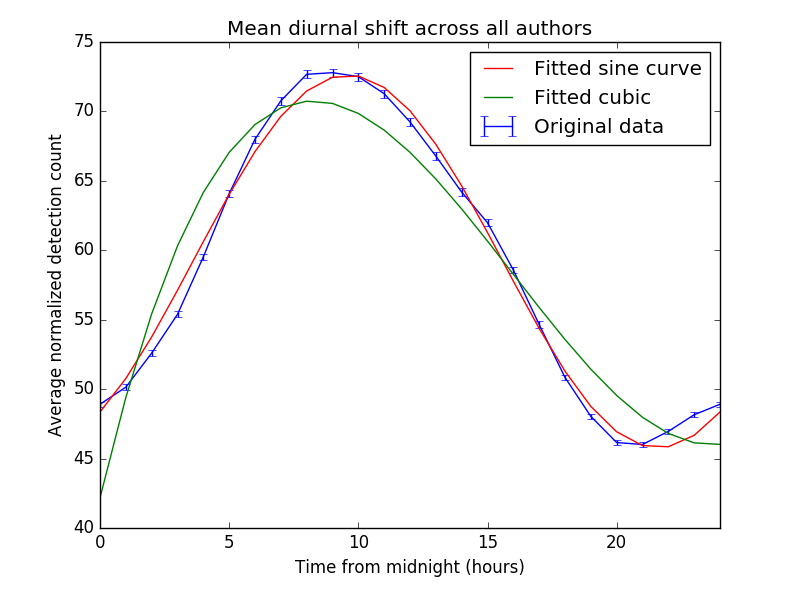
\includegraphics[width=\linewidth]{dishift/diurnal_shift_fit}
	\caption{Diurnal shift across all authors \& sine-function fit
		\label{fig:dishift:fit}}
\end{figure}

Figure~\ref{fig:dishift:all} shows the same graph as figure~\ref{fig:dishift:fit} (for comparison), as well as diurnal shift curves for each respective location. Surprisingly, each location category shows a sine curve. The peak of these sine curves appears to be correlated well with latitude. The average longitudes in degrees are, for Europe, Asia \& Australia, and North America respectively: $\sim 15$, $\sim 150$ \& $\sim -100$. This supports the idea of a sine-function describing the diurnal shift, since larger longitudes produce a greater hour of diurnal shift, bearing in mind that the hour for the North American categoryw ill `wrap' around, due to timezones. The average latitudes in degrees are (respectively): $\sim 45$, $\sim 35$ \& $\sim 15$. The North American category has the largest intensity, followed by the European category and then Asia \& Australia, though this is not the order of latitudes. This appears to disagree with research noted in section~\ref{sec:dishift:litrev}, which suggested that the intensity (amplitude) of diurnal shift is dependent on latitude.  

\begin{figure}[h!]
	\centering
	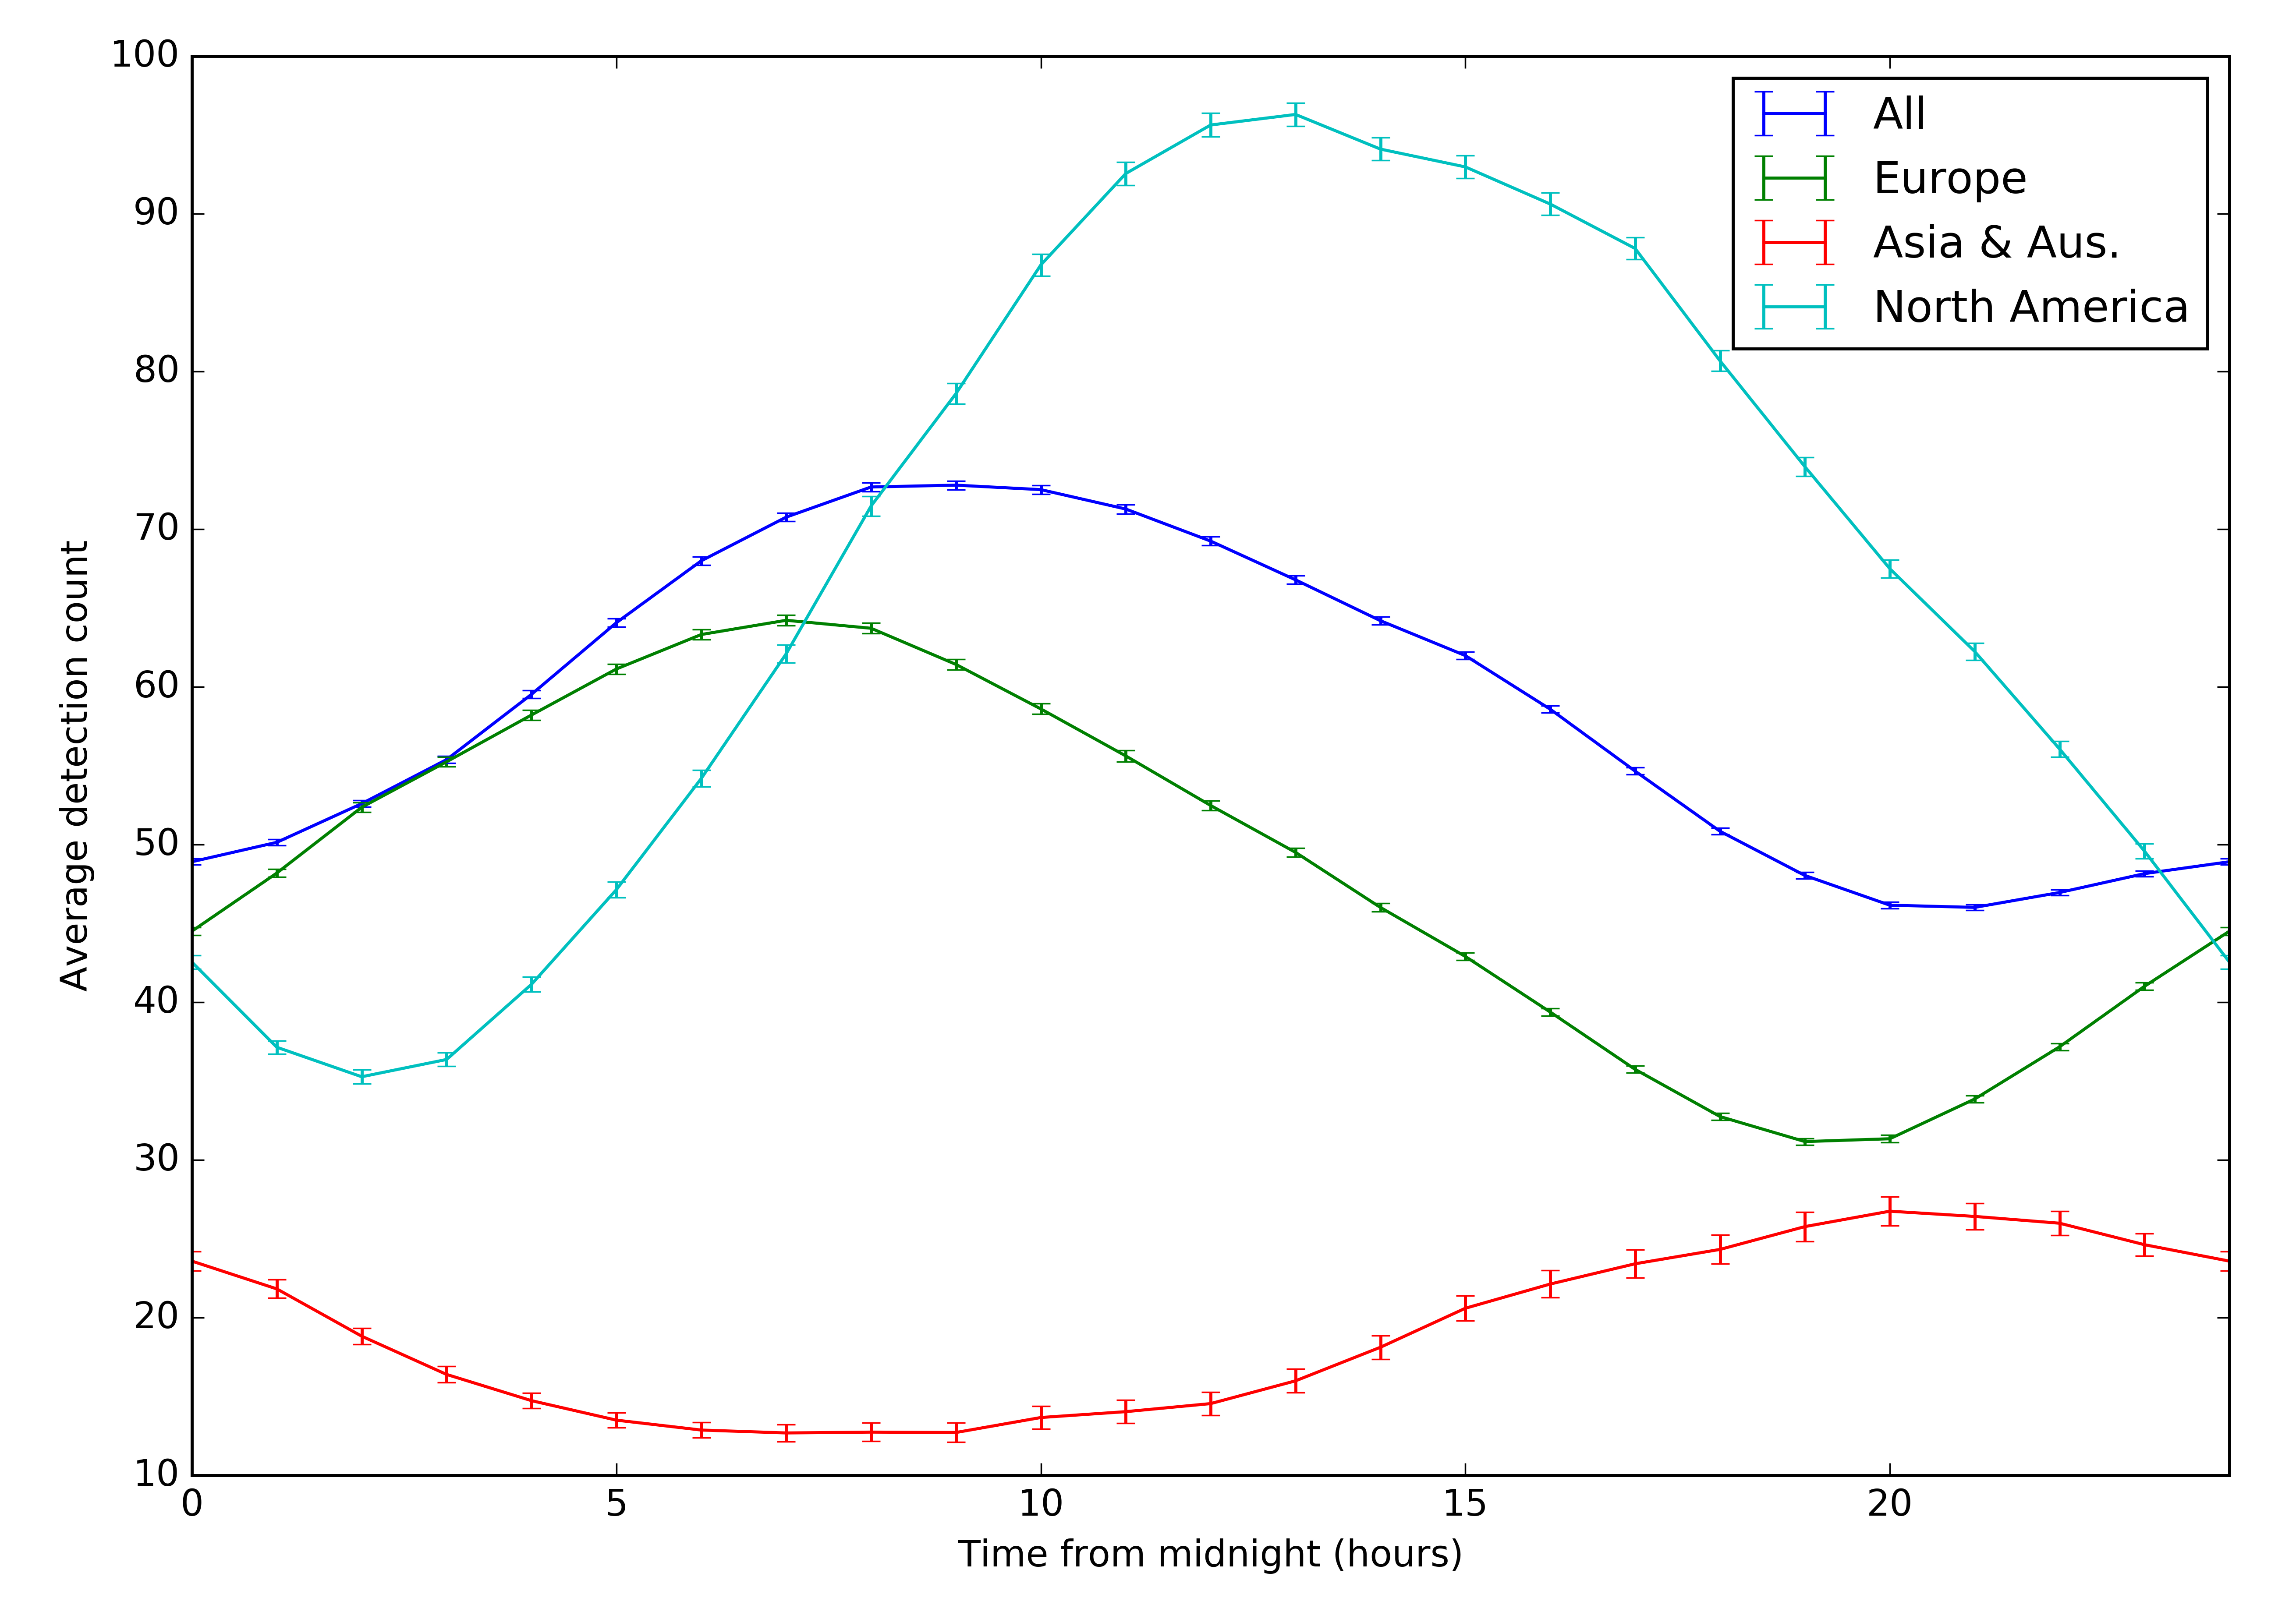
\includegraphics[width=\linewidth]{dishift/all_shifts}
	\caption{Diurnal shifts for each individual location (all observers' shift included for reference)
		\label{fig:dishift:all}}
\end{figure}

The sum of parameter covariances for each location category are shown below. The positive numbers all indicate a positive correlation, as expected from the figures. 
\begin{table}[h!]
	\begin{tabular}{ccccc}
		\hline
		Category & $A$ & $\phi$ & $\mu$ & Covar. \\ \hline
		All & 13.4 & -0.941 & 59.2 & 0.454 \\
		Europe & 15.4 & -0.302 & 48.4 & 0.498 \\
		Asia \& Aus. & -7.19 & -0.585 & 19.0 & 0.352 \\
		N. America & 29.5 & -2.05 & 68.1 & 1.16 \\
		\hline
	\end{tabular}
	\caption{Sum of parameter covariances for each location category}
\end{table}

\subsection{Spatial variation}
Created using QGIS, I present a map showing the location of each observer in the data set. The dot for each circle is coloured (as in the legend) based on the peak hour of the diurnal shift. This gives a more visual demonstration of what is shown in figures~\ref{fig:dishift:all} and \ref{fig:dishift:lon:peak}: the colours are clearly grouped based on location. Observers in Europe have diurnal shift peaks mostly around 6:00, North American observers have peaks around 15:00 and in Asia \& Australia around 20. This supports implications from the previously stated figures. There are clearly anomalous results for some observers (note the blue dots in Europe), though this is expected.
\begin{figure}[h!]
	\centering
	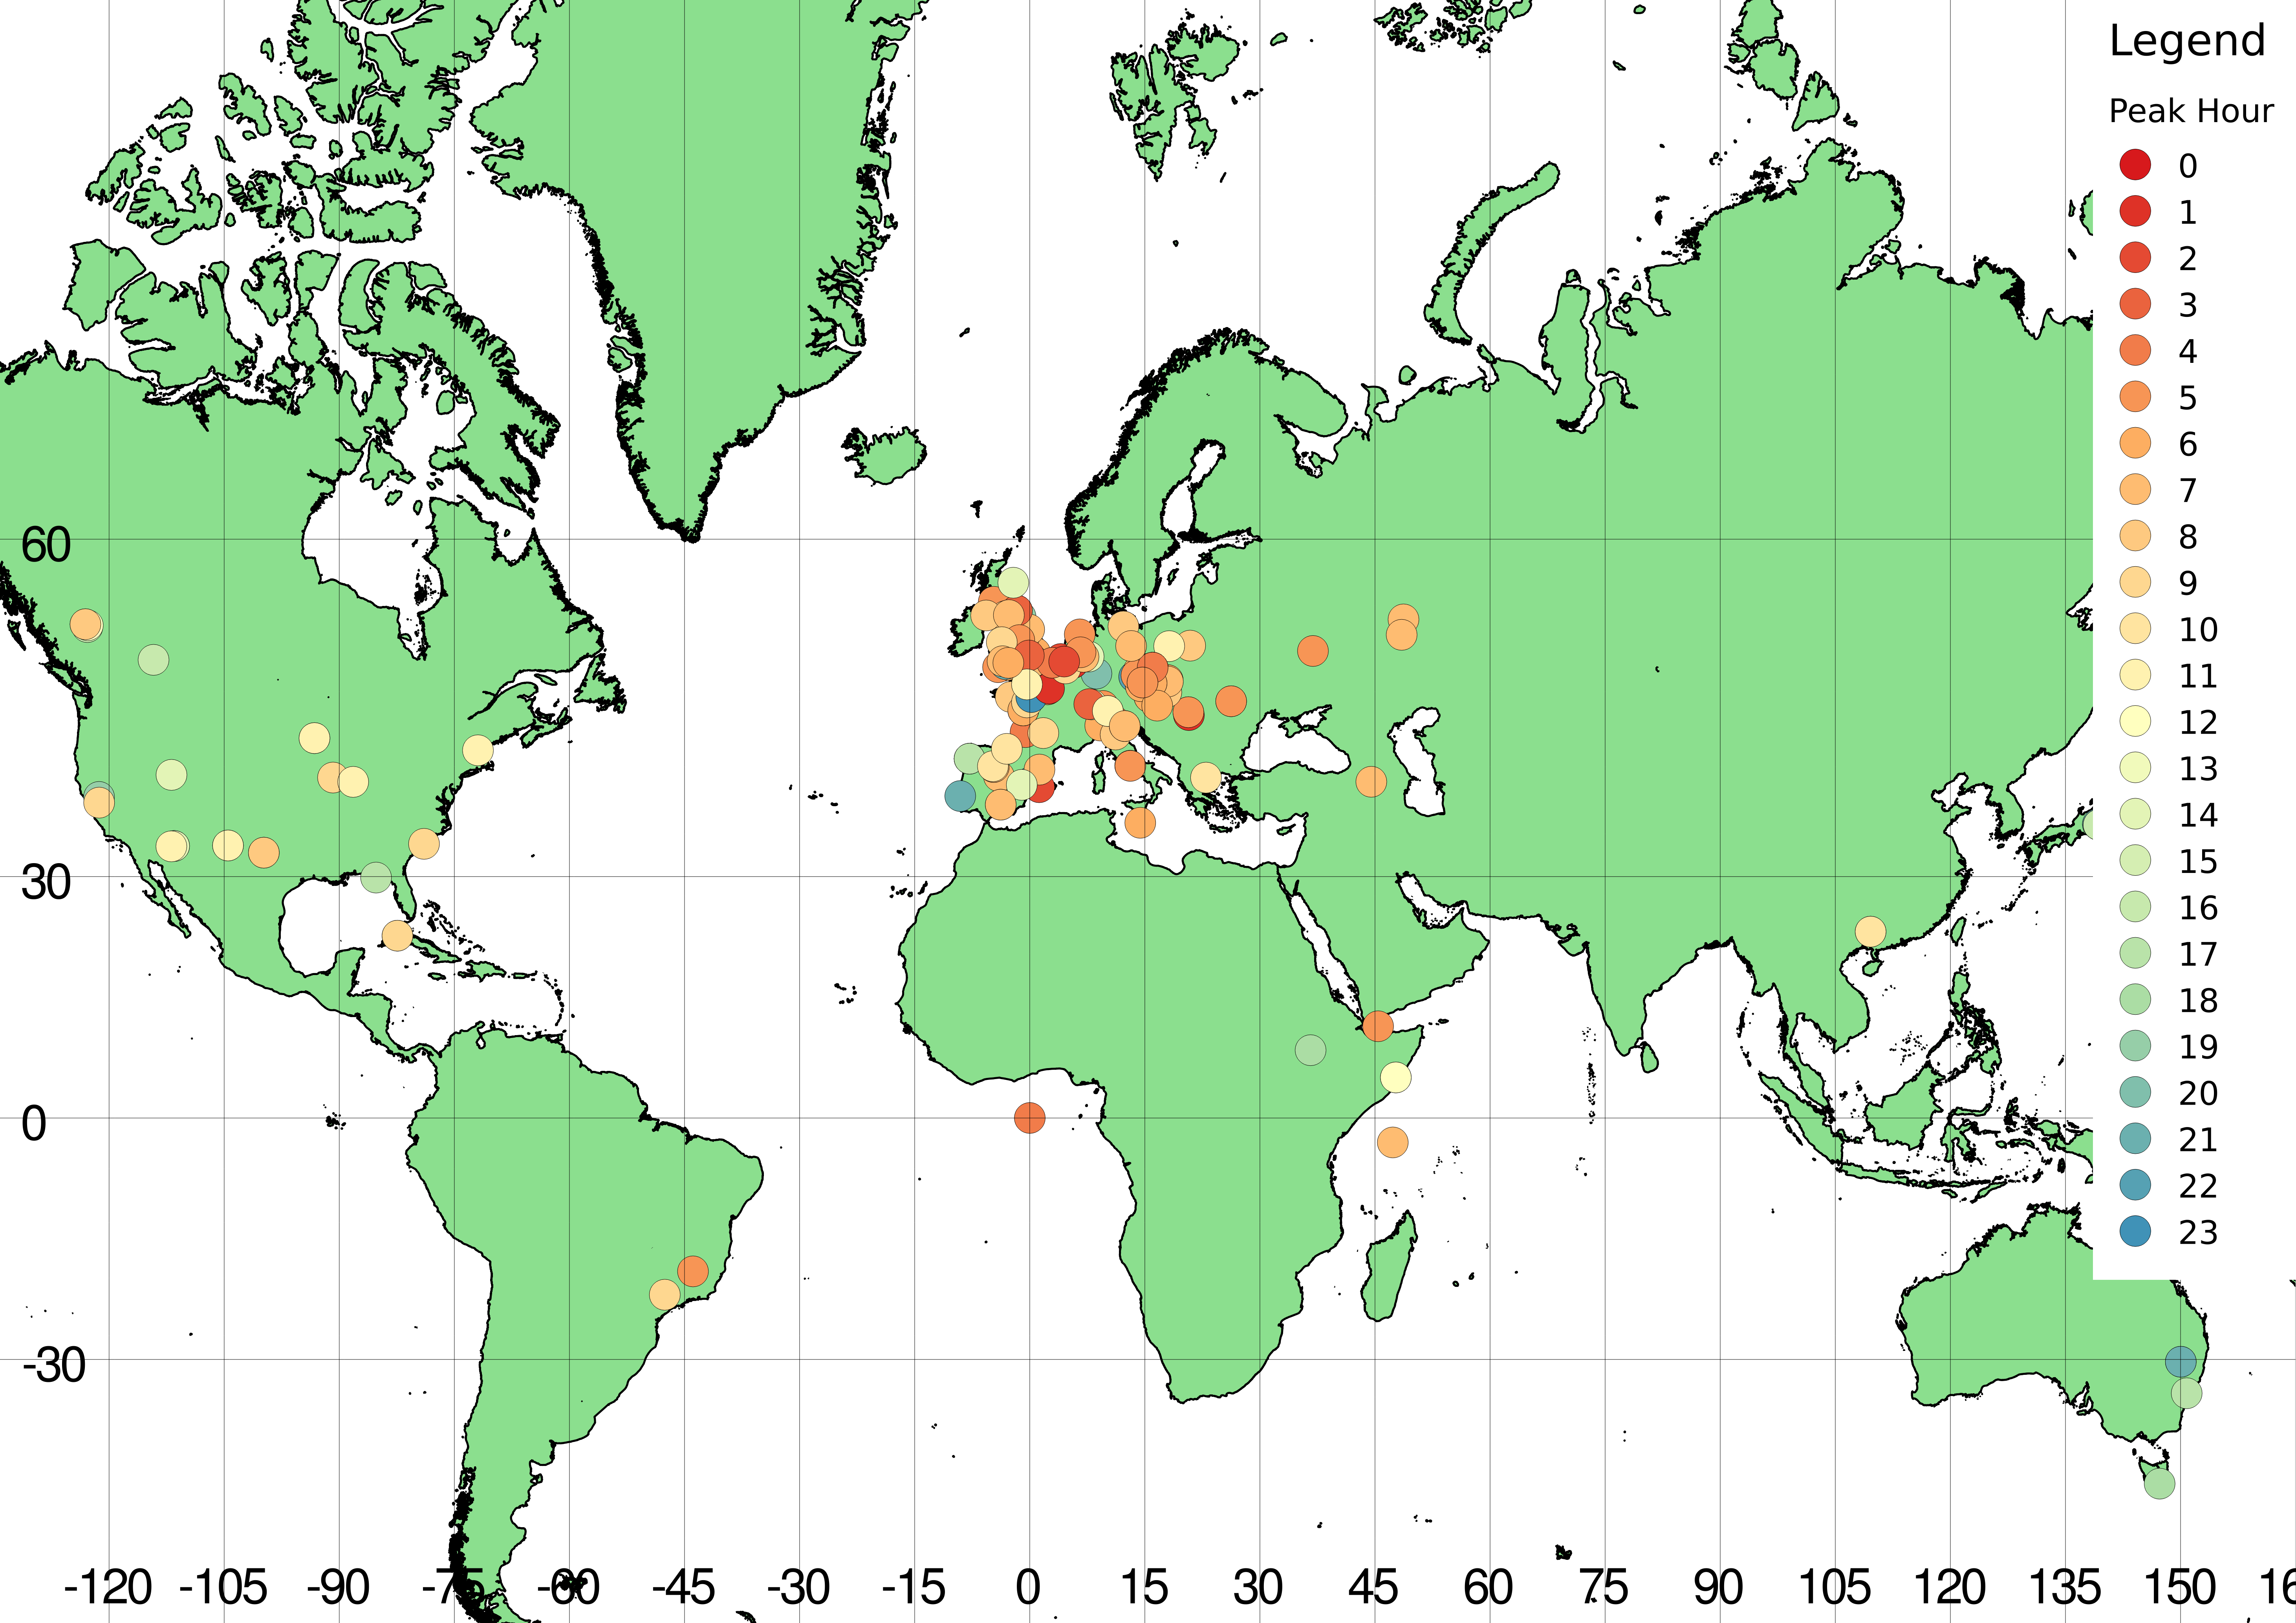
\includegraphics[width=\linewidth]{dishift/peak_qgis}
	\caption{Peak hour of diurnal shift for each observer
		\label{fig:dishift:qgis}}
\end{figure}
\paragraph{Latitude\\}
There appears to be little correlation between latitude and the peak hour. Although, overall, the hour appears to decrease as the latitude varies from $-40^{\circ}$ to $60^{\circ}$, there errors are substantial. The implication of this is there is little agreement within each category, suggesting no correlation at all. However, this is expected. There is no logical reason why the peak hour would be influenced by the latitude. Diurnal shift is caused (according to my model and \cite{baa}) by the Earth's rotation changing the average incident velocity of meteors. This does not change with latitude, hence no correlation is seen.
\begin{figure}[h!]
	\centering
	\includegraphics[width=\linewidth]{spatial/latitude/peak}
	\caption{Peak hour of diurnal shift against latitude
		\label{fig:dishift:lat:peak}}
\end{figure}

In figure~\ref{fig:dishift:lat:fit} little correlation is seen again. The covariances vary widely. There is no clear trend, suggesting that the latitude of an observer has no effect on how well data fits a sine function. Consequently, it would appear that diurnal shift is a global phenomenon.
\begin{figure}[h!]
	\centering
	\includegraphics[width=\linewidth]{spatial/latitude/fit}
	\caption{Optimal sine function fit against latitude
		\label{fig:dishift:lat:fit}}
\end{figure}

\paragraph{Longitude\\}
Figure~\ref{fig:dishift:lon:peak} shows agreement with figures~\ref{fig:dishift:all} and \ref{fig:dishift:qgis}. The peak hour is lowest for a longitude of $0^{\circ}$ and increases either side of this, as seen in the stated figures. The errors for some categories are reasonably large, though still fall in a range that fits the trend. There is, of course, minor variation though the trend is clear from the data: latitude and peak hour of diurnal shift are related.
\begin{figure}[h!]
	\centering
	\includegraphics[width=\linewidth]{spatial/longitude/peak}
	\caption{Peak hour of diurnal shift against longitude
		\label{fig:dishift:lon:peak}}
\end{figure}\\
In order to investigate this apparent trend further, I have corrected the peak hour of each location category such that $H_{\text{corrected}} = H_{\text{calculated}} + \frac{\phi}{15}$, provided the longitude $\phi$ is in degrees. This means that the hour will be the local time (not using timezones, only the time based on longitude). This is shown in figure~\ref{fig:dishift:lon:corrected}. Errorbars, in this case, are such that 75\% of the data for a given location category falls within the bars. The values appear to fluctuate around a peak hour of 6am (shown in green), supporting the model I have proposed. However, there is a large degree of variation.
\begin{figure}[h!]
	\centering
	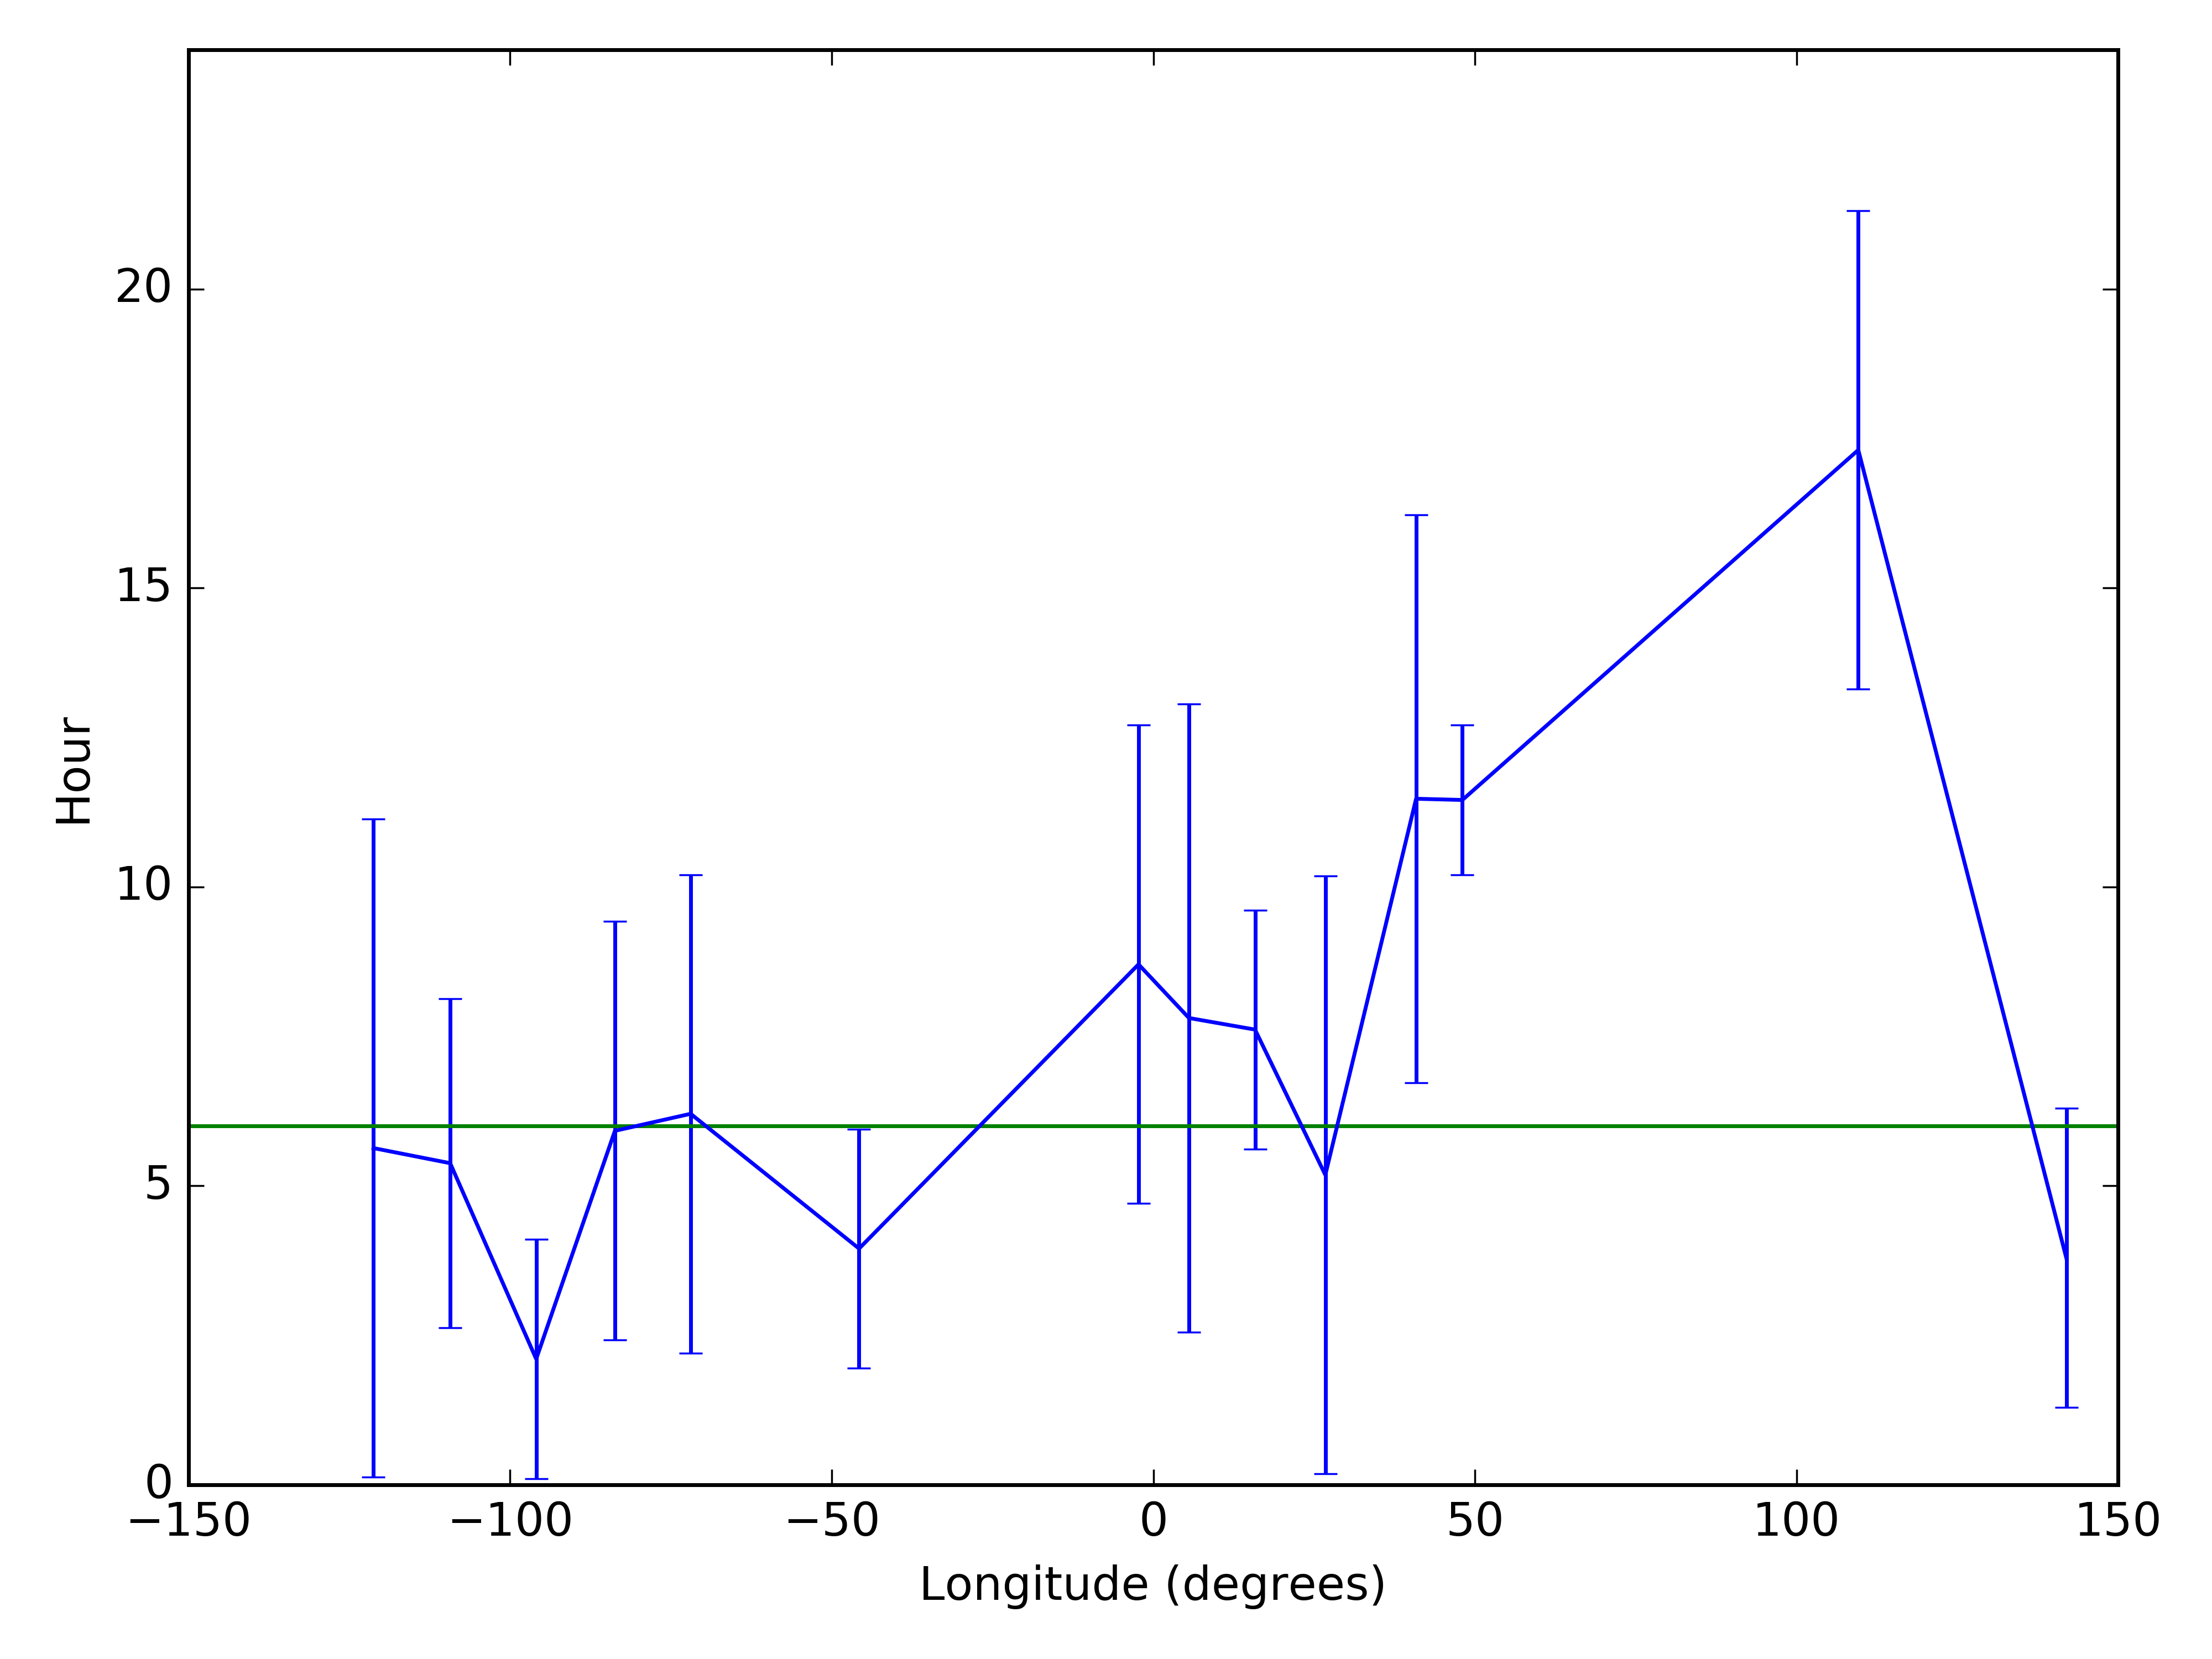
\includegraphics[width=\linewidth]{spatial/longitude/corrected}
	\caption{Corrected peak hour of diurnal shift against longitude
		\label{fig:dishift:lon:corrected}}
\end{figure}\\
In figure~\ref{fig:dishift:lon:hist} a histogram of the peak hour is shown. It is clear from this figure that the model is supported. Clearly most of the observers have a peak hour around 6, with some having a peak hour of 7. This is reasonable; as noted in section~\ref{sec:dishift:model}, the peak hour can in fact be slightly after 6am, since changes in the ionosphere occur around this time, as the Sun comes over the horizon. This can improve radio detection, allowing for better conditions that would shift the peak hour. Of course, there is some distribution either side of 6am, though this is expected.
\begin{figure}[h!]
	\centering
	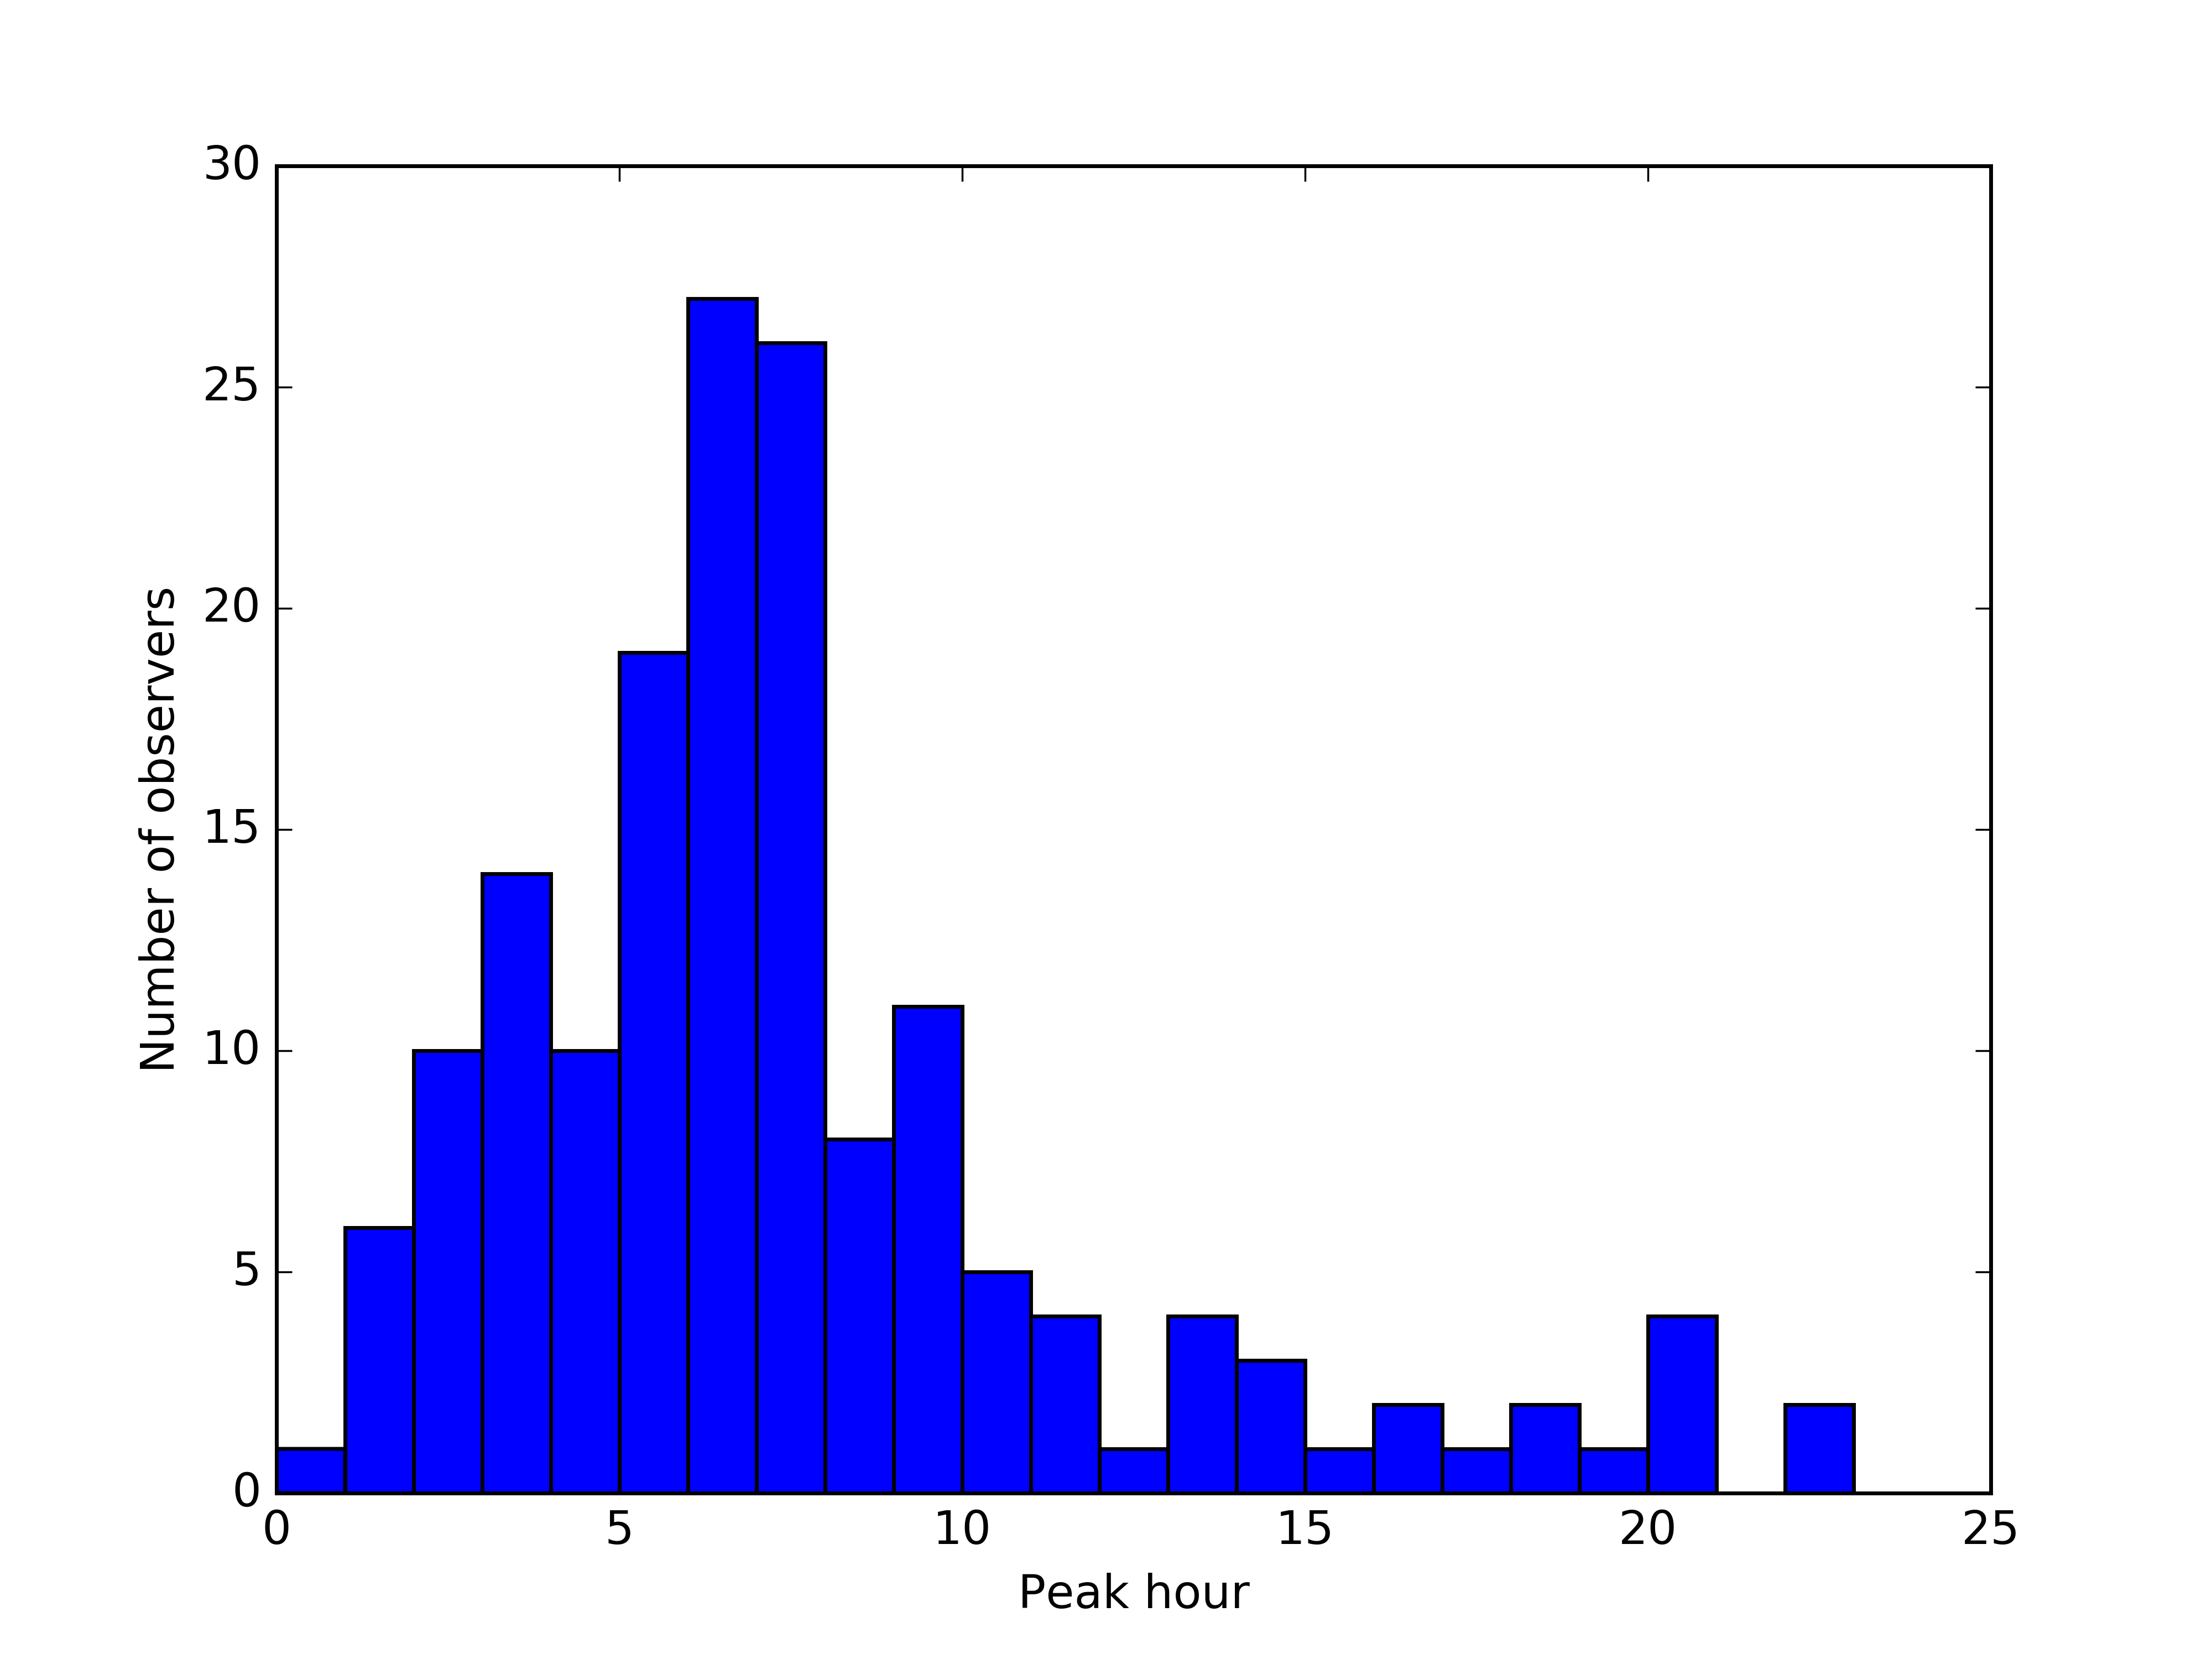
\includegraphics[width=\linewidth]{spatial/longitude/hist}
	\caption{Histogram of peak hours
		\label{fig:dishift:lon:hist}}
\end{figure}

The covariance varies a small amount with longitude other than a few categories. There does not appear to be a clear trend.  However, the poorest fits have large errors indicating that this is not a poor fit throughout observers in said categories. Consequently it would seem that the fit varies moderately across the globe. 
\begin{figure}[h!]
	\centering
	\includegraphics[width=\linewidth]{spatial/longitude/fit}
	\caption{Optimal sine function fit against longitude
		\label{fig:dishift:lon:fit}}
\end{figure}


\subsection{Temporal variation}
Figure~\ref{fig:dishift:temp:peak} shows the same result as previously noted. The variation for each location category varies around the hours expected if peak hour is correlated with longitude. There is a large amount of variation for the Asia \& Australia category, so it is hard to make an analysis from this. It is clear that in more recent years, there is less variation. Over time, no categories appear to increase or decrease, but instead fluctuate around certain values.
\begin{figure}[h!]
	\centering
	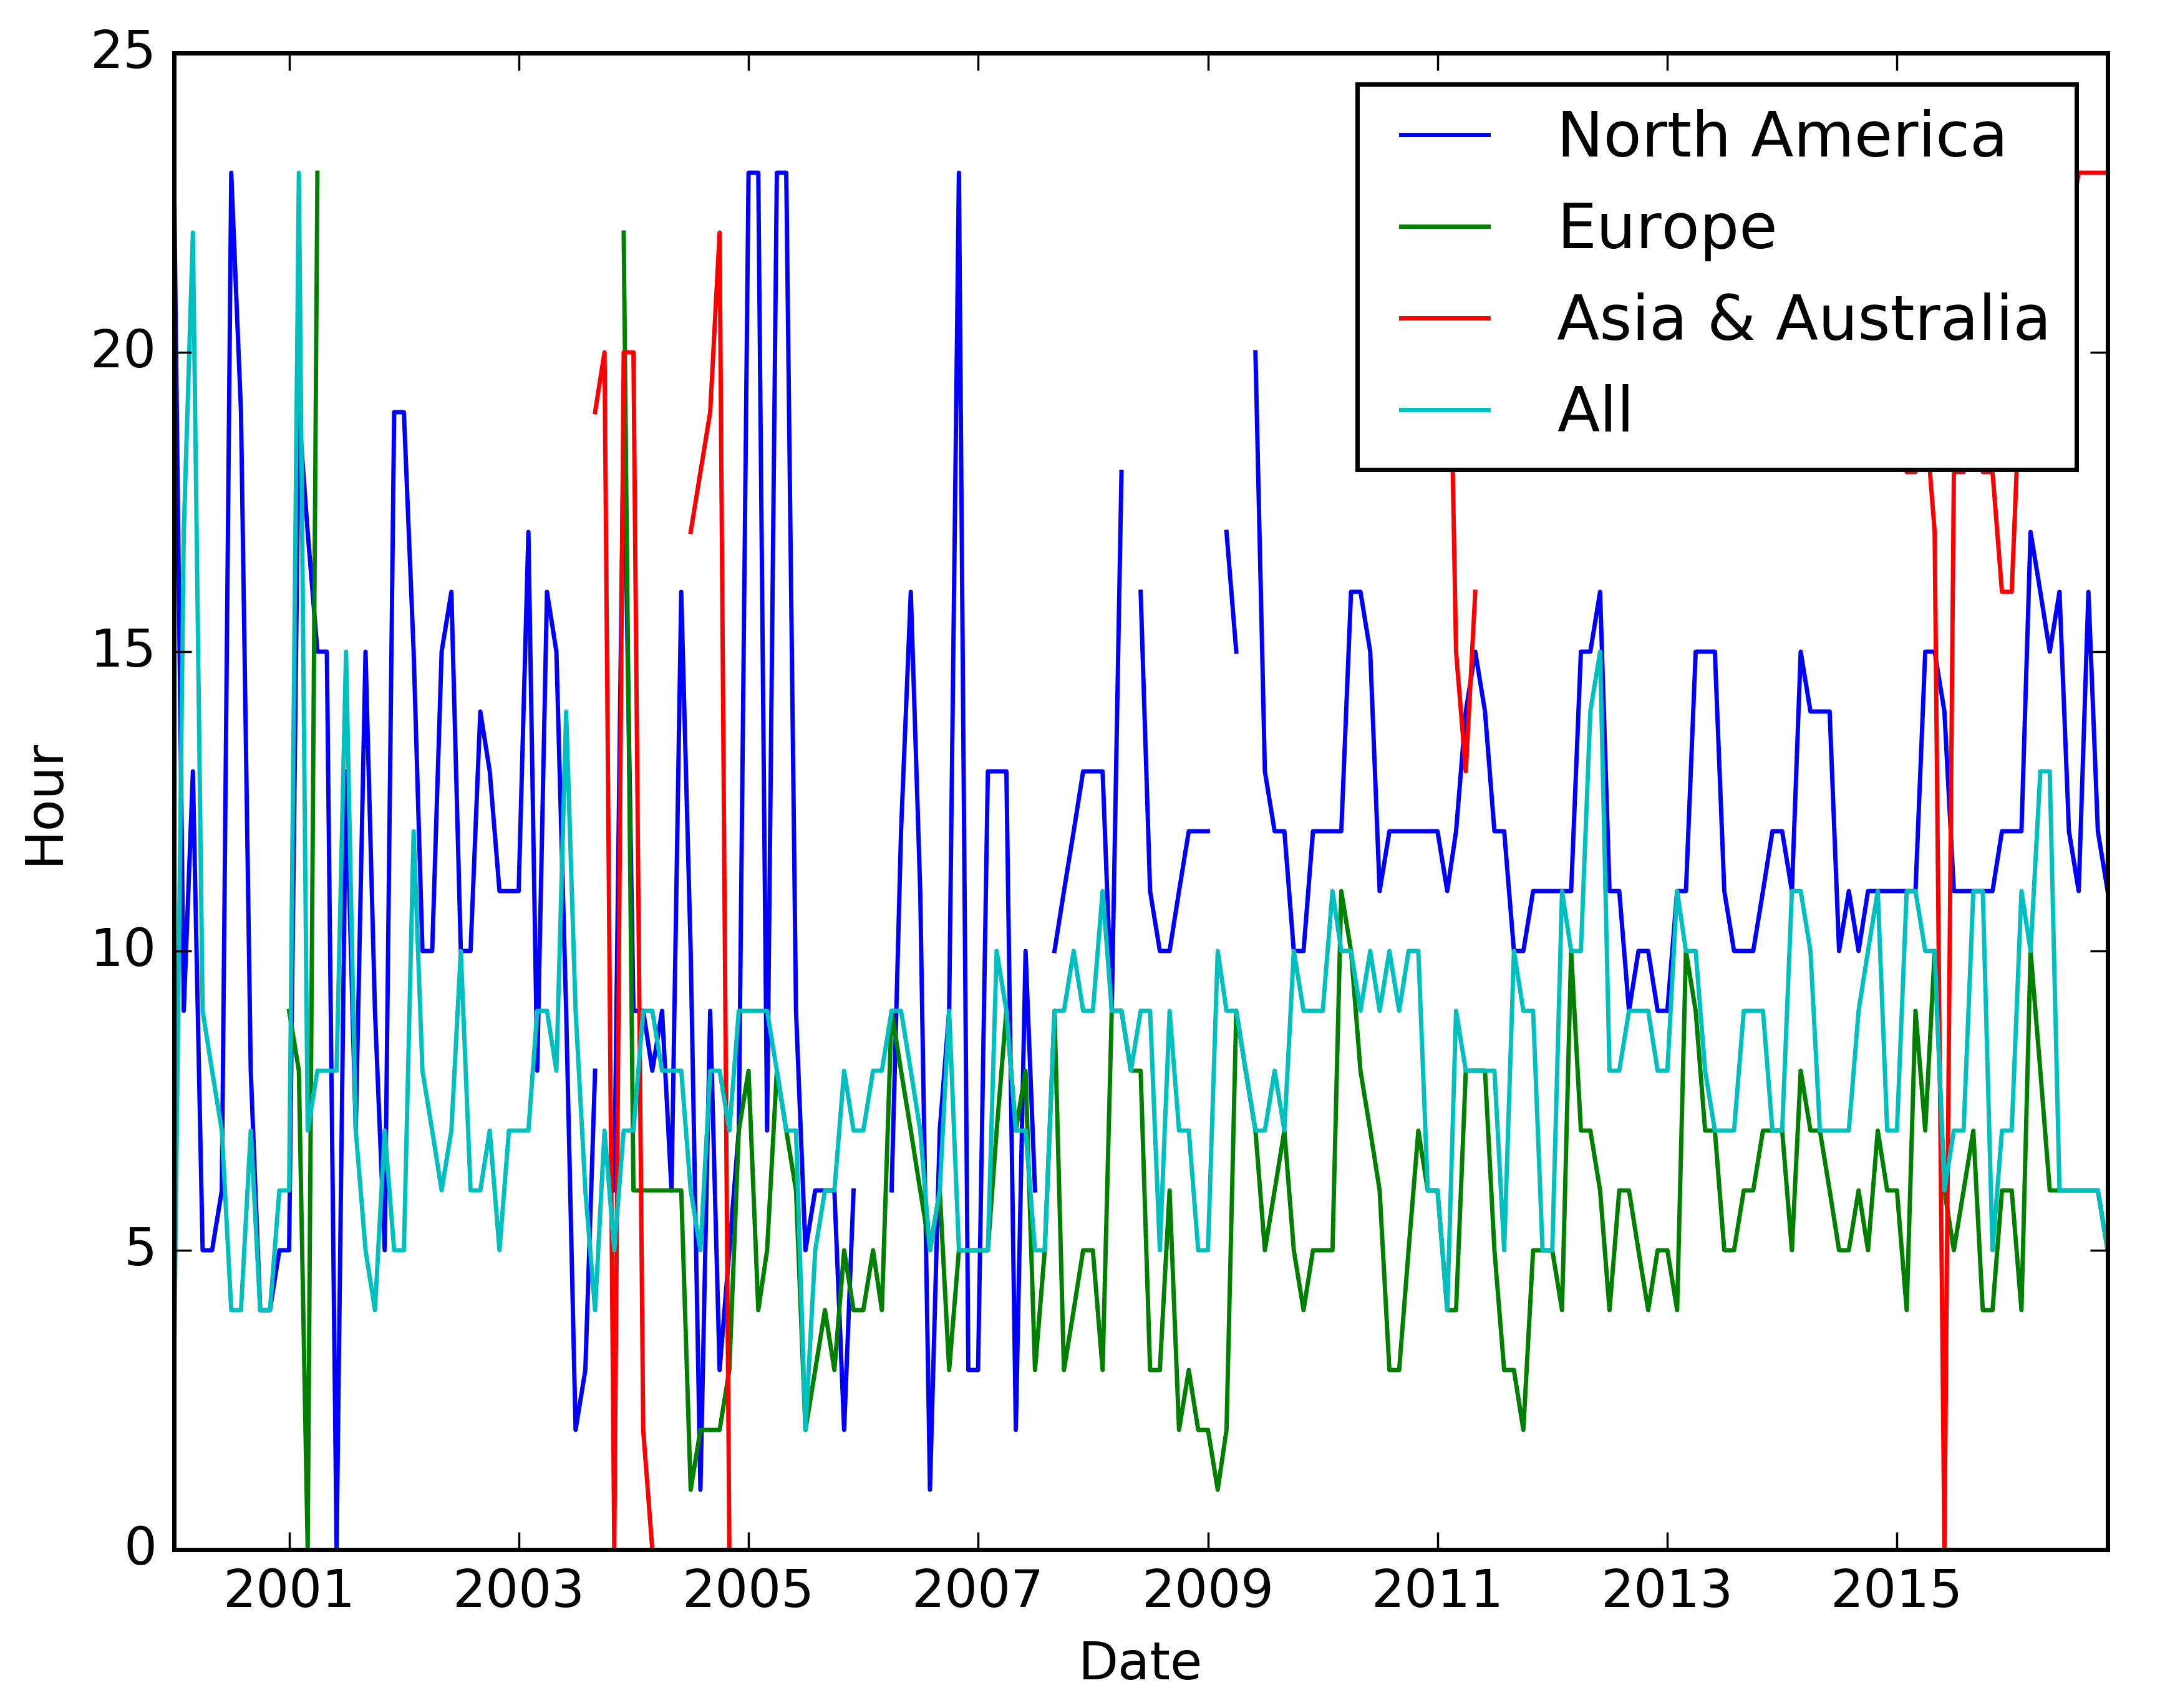
\includegraphics[width=\linewidth]{temporal/analyses/COMBINEDpeak}
	\caption{Peak hour of diurnal shift change over time
		\label{fig:dishift:temp:peak}}
\end{figure}
Generally, the fit is reasonably good. Between 2005 and 2011, the fits are much worse, indicating either a weaker diurnal shift (an unlikely phenomenon) or a more intense background level. For periods outside this, there is a low value of variation. All categories have a similar fit and absent trend over time.
\begin{figure}[h!]
	\centering
	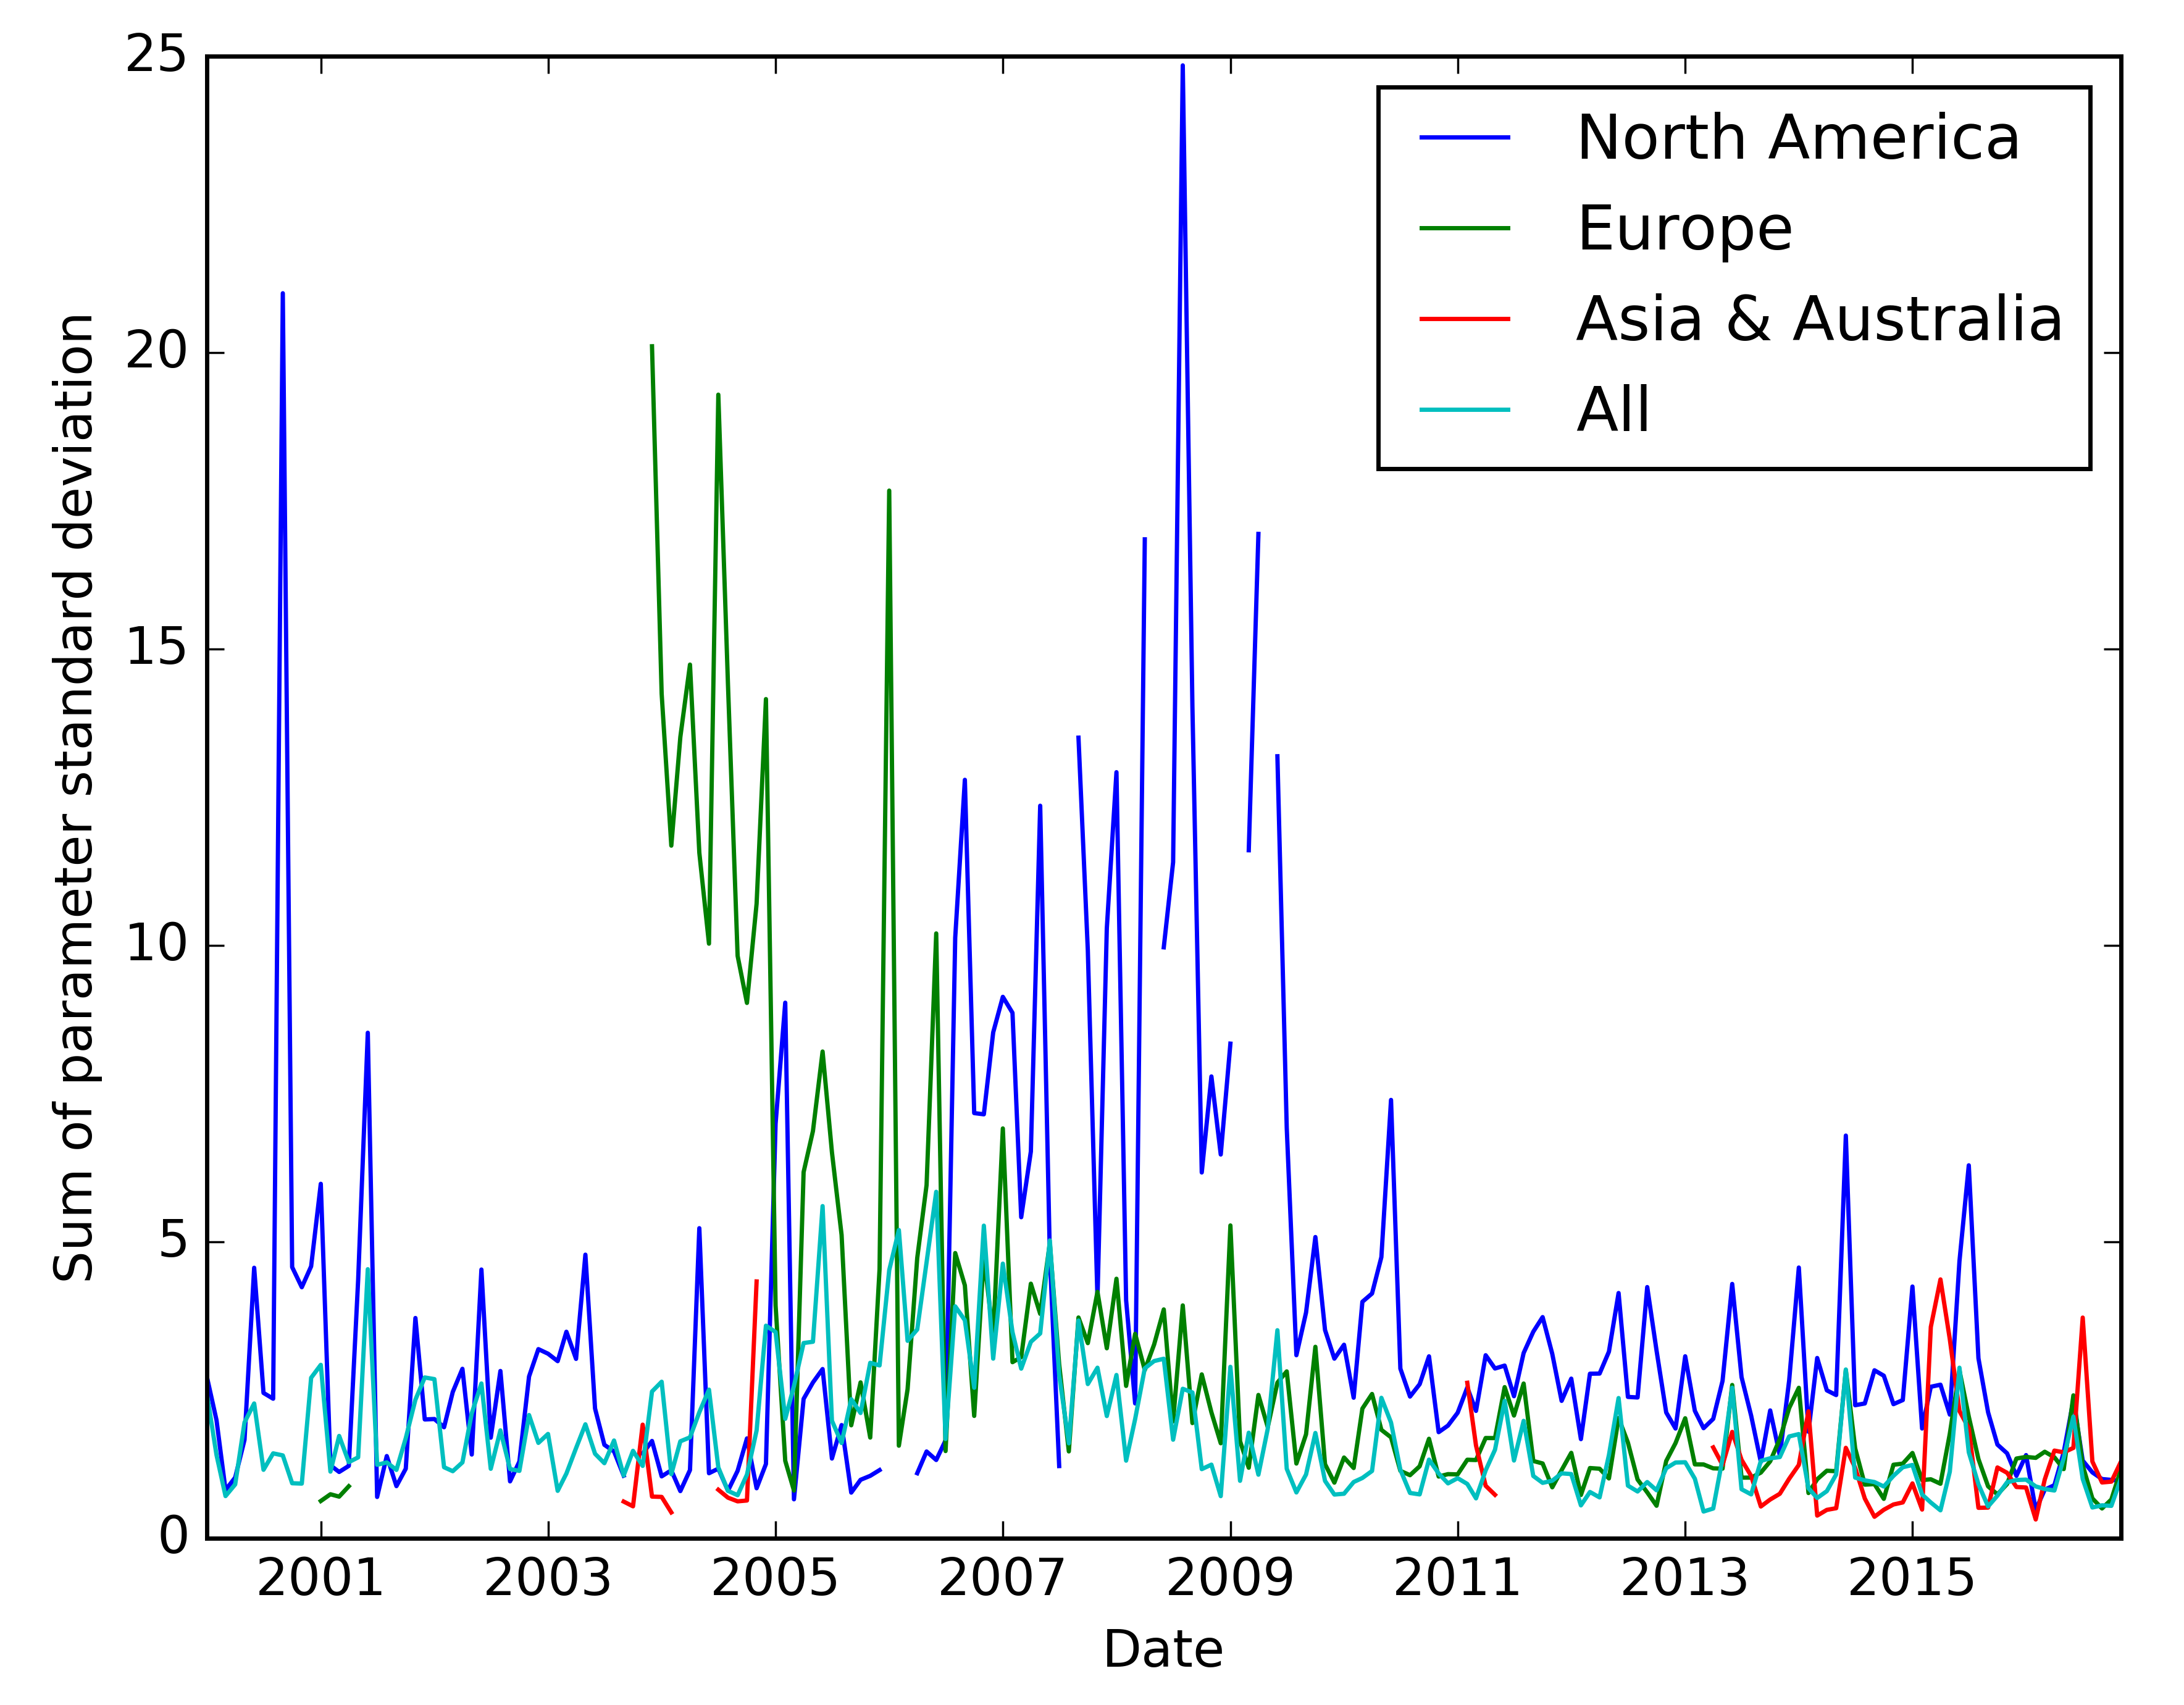
\includegraphics[width=\linewidth]{temporal/analyses/COMBINEDfit}
	\caption{Optimal sine function fit change over time
		\label{fig:dishift:temp:fit}}
\end{figure}
\subsection{Improvements}
\paragraph{Annual variation\\}
A question, that may reveal more information on the processes behind diurnal shift, is whether the phenomenon changes on a yearly time scale. Seasonal variation of diurnal shift may indicate an influence from sources such as the Sun, or the orientation of the Earth relative to it's orbit.
\paragraph{Intensity variation with latitude\\}
Singer, W., von Zahn, U., Batista, P. P., Fuller, B., \& Latteck, R. \cite{latitudes} analyse a variation of diurnal shift amplitude with latitude. Their analysis is over a relatively small range of latitudes. A further investigation, with a wider range of latitudes and more observers involved, could confirm or support their analysis. My own analysis indicates that there is little correlation.
\paragraph{Receiving station vs. detection station}
Most meteor detection setups are simply receiving stations. Typically a station, often a considerable distance away, emits a signal that reflects off of the meteor's ionised trail and is received by the observers, whose data are under consideration. This means that there is a difference between the longitude of the observer and the longitude of where the detection takes place. This will, of course, influence the conclusions made. Were the longitude of each detection station known, it may further support the conclusions of my model.
\section{Conclusion}
There is a clear correlation between longitude and peak hour of diurnal shift, as suggested by the model I propose. This is apparent from several results, including a histogram of peak hours. This good agreement indicates that my model is valid and is supported by the data. In addition, based on this analysis and previous analyses, it seems that there is little correlation between location and a sine function fit, suggesting that the intensity of diurnal shift (in the sense of relative intensity compared to background rates) is roughly uniform across the globe. However, there is no clear link to be made between the amplitude of diurnal shift and latitude. There appears to be a correlation, in general, with location, with a clear difference in amplitude between different location categories.